% Options for packages loaded elsewhere
\PassOptionsToPackage{unicode}{hyperref}
\PassOptionsToPackage{hyphens}{url}
%
\documentclass[
  man,floatsintext]{apa6}
\usepackage{amsmath,amssymb}
\usepackage{lmodern}
\usepackage{iftex}
\ifPDFTeX
  \usepackage[T1]{fontenc}
  \usepackage[utf8]{inputenc}
  \usepackage{textcomp} % provide euro and other symbols
\else % if luatex or xetex
  \usepackage{unicode-math}
  \defaultfontfeatures{Scale=MatchLowercase}
  \defaultfontfeatures[\rmfamily]{Ligatures=TeX,Scale=1}
\fi
% Use upquote if available, for straight quotes in verbatim environments
\IfFileExists{upquote.sty}{\usepackage{upquote}}{}
\IfFileExists{microtype.sty}{% use microtype if available
  \usepackage[]{microtype}
  \UseMicrotypeSet[protrusion]{basicmath} % disable protrusion for tt fonts
}{}
\makeatletter
\@ifundefined{KOMAClassName}{% if non-KOMA class
  \IfFileExists{parskip.sty}{%
    \usepackage{parskip}
  }{% else
    \setlength{\parindent}{0pt}
    \setlength{\parskip}{6pt plus 2pt minus 1pt}}
}{% if KOMA class
  \KOMAoptions{parskip=half}}
\makeatother
\usepackage{xcolor}
\IfFileExists{xurl.sty}{\usepackage{xurl}}{} % add URL line breaks if available
\IfFileExists{bookmark.sty}{\usepackage{bookmark}}{\usepackage{hyperref}}
\hypersetup{
  pdftitle={An Item Response Theory based open-source online assessment of vocabulary skills in 3 to 8-year-old children},
  pdfauthor={Manuel Bohn1, Julia Prein1, Daniel Haun1, \& Natalia Gagarina2},
  pdflang={en-EN},
  pdfkeywords={keywords},
  hidelinks,
  pdfcreator={LaTeX via pandoc}}
\urlstyle{same} % disable monospaced font for URLs
\usepackage{graphicx}
\makeatletter
\def\maxwidth{\ifdim\Gin@nat@width>\linewidth\linewidth\else\Gin@nat@width\fi}
\def\maxheight{\ifdim\Gin@nat@height>\textheight\textheight\else\Gin@nat@height\fi}
\makeatother
% Scale images if necessary, so that they will not overflow the page
% margins by default, and it is still possible to overwrite the defaults
% using explicit options in \includegraphics[width, height, ...]{}
\setkeys{Gin}{width=\maxwidth,height=\maxheight,keepaspectratio}
% Set default figure placement to htbp
\makeatletter
\def\fps@figure{htbp}
\makeatother
\setlength{\emergencystretch}{3em} % prevent overfull lines
\providecommand{\tightlist}{%
  \setlength{\itemsep}{0pt}\setlength{\parskip}{0pt}}
\setcounter{secnumdepth}{-\maxdimen} % remove section numbering
% Make \paragraph and \subparagraph free-standing
\ifx\paragraph\undefined\else
  \let\oldparagraph\paragraph
  \renewcommand{\paragraph}[1]{\oldparagraph{#1}\mbox{}}
\fi
\ifx\subparagraph\undefined\else
  \let\oldsubparagraph\subparagraph
  \renewcommand{\subparagraph}[1]{\oldsubparagraph{#1}\mbox{}}
\fi
\newlength{\cslhangindent}
\setlength{\cslhangindent}{1.5em}
\newlength{\csllabelwidth}
\setlength{\csllabelwidth}{3em}
\newlength{\cslentryspacingunit} % times entry-spacing
\setlength{\cslentryspacingunit}{\parskip}
\newenvironment{CSLReferences}[2] % #1 hanging-ident, #2 entry spacing
 {% don't indent paragraphs
  \setlength{\parindent}{0pt}
  % turn on hanging indent if param 1 is 1
  \ifodd #1
  \let\oldpar\par
  \def\par{\hangindent=\cslhangindent\oldpar}
  \fi
  % set entry spacing
  \setlength{\parskip}{#2\cslentryspacingunit}
 }%
 {}
\usepackage{calc}
\newcommand{\CSLBlock}[1]{#1\hfill\break}
\newcommand{\CSLLeftMargin}[1]{\parbox[t]{\csllabelwidth}{#1}}
\newcommand{\CSLRightInline}[1]{\parbox[t]{\linewidth - \csllabelwidth}{#1}\break}
\newcommand{\CSLIndent}[1]{\hspace{\cslhangindent}#1}
\ifLuaTeX
\usepackage[bidi=basic]{babel}
\else
\usepackage[bidi=default]{babel}
\fi
\babelprovide[main,import]{english}
% get rid of language-specific shorthands (see #6817):
\let\LanguageShortHands\languageshorthands
\def\languageshorthands#1{}
% Manuscript styling
\usepackage{upgreek}
\captionsetup{font=singlespacing,justification=justified}

% Table formatting
\usepackage{longtable}
\usepackage{lscape}
% \usepackage[counterclockwise]{rotating}   % Landscape page setup for large tables
\usepackage{multirow}		% Table styling
\usepackage{tabularx}		% Control Column width
\usepackage[flushleft]{threeparttable}	% Allows for three part tables with a specified notes section
\usepackage{threeparttablex}            % Lets threeparttable work with longtable

% Create new environments so endfloat can handle them
% \newenvironment{ltable}
%   {\begin{landscape}\begin{center}\begin{threeparttable}}
%   {\end{threeparttable}\end{center}\end{landscape}}
\newenvironment{lltable}{\begin{landscape}\begin{center}\begin{ThreePartTable}}{\end{ThreePartTable}\end{center}\end{landscape}}

% Enables adjusting longtable caption width to table width
% Solution found at http://golatex.de/longtable-mit-caption-so-breit-wie-die-tabelle-t15767.html
\makeatletter
\newcommand\LastLTentrywidth{1em}
\newlength\longtablewidth
\setlength{\longtablewidth}{1in}
\newcommand{\getlongtablewidth}{\begingroup \ifcsname LT@\roman{LT@tables}\endcsname \global\longtablewidth=0pt \renewcommand{\LT@entry}[2]{\global\advance\longtablewidth by ##2\relax\gdef\LastLTentrywidth{##2}}\@nameuse{LT@\roman{LT@tables}} \fi \endgroup}

% \setlength{\parindent}{0.5in}
% \setlength{\parskip}{0pt plus 0pt minus 0pt}

% Overwrite redefinition of paragraph and subparagraph by the default LaTeX template
% See https://github.com/crsh/papaja/issues/292
\makeatletter
\renewcommand{\paragraph}{\@startsection{paragraph}{4}{\parindent}%
  {0\baselineskip \@plus 0.2ex \@minus 0.2ex}%
  {-1em}%
  {\normalfont\normalsize\bfseries\itshape\typesectitle}}

\renewcommand{\subparagraph}[1]{\@startsection{subparagraph}{5}{1em}%
  {0\baselineskip \@plus 0.2ex \@minus 0.2ex}%
  {-\z@\relax}%
  {\normalfont\normalsize\itshape\hspace{\parindent}{#1}\textit{\addperi}}{\relax}}
\makeatother

% \usepackage{etoolbox}
\makeatletter
\patchcmd{\HyOrg@maketitle}
  {\section{\normalfont\normalsize\abstractname}}
  {\section*{\normalfont\normalsize\abstractname}}
  {}{\typeout{Failed to patch abstract.}}
\patchcmd{\HyOrg@maketitle}
  {\section{\protect\normalfont{\@title}}}
  {\section*{\protect\normalfont{\@title}}}
  {}{\typeout{Failed to patch title.}}
\makeatother

\usepackage{xpatch}
\makeatletter
\xapptocmd\appendix
  {\xapptocmd\section
    {\addcontentsline{toc}{section}{\appendixname\ifoneappendix\else~\theappendix\fi\\: #1}}
    {}{\InnerPatchFailed}%
  }
{}{\PatchFailed}
\keywords{keywords\newline\indent Word count: X}
\usepackage{lineno}

\linenumbers
\usepackage{csquotes}
\ifLuaTeX
  \usepackage{selnolig}  % disable illegal ligatures
\fi

\title{An Item Response Theory based open-source online assessment of vocabulary skills in 3 to 8-year-old children}
\author{Manuel Bohn\textsuperscript{1}, Julia Prein\textsuperscript{1}, Daniel Haun\textsuperscript{1}, \& Natalia Gagarina\textsuperscript{2}}
\date{}


\shorttitle{Vocabulary assessment in 3 to 8-year-old children}

\authornote{

We thank Susanne Mauritz for help with the data collection.

The authors made the following contributions. Manuel Bohn: Conceptualization, Formal Analysis, Writing - Original Draft Preparation, Writing - Review \& Editing; Julia Prein: Conceptualization, Software, Writing - Original Draft Preparation, Writing - Review \& Editing; Daniel Haun: Conceptualization, Writing - Review \& Editing; Natalia Gagarina: Conceptualization, Writing - Original Draft Preparation, Writing - Review \& Editing.

Correspondence concerning this article should be addressed to Manuel Bohn, Max Planck Institute for Evolutionary Anthropology, Deutscher Platz 6, 04103 Leipzig, Germany. E-mail: \href{mailto:manuel_bohn@eva.mpg.de}{\nolinkurl{manuel\_bohn@eva.mpg.de}}

}

\affiliation{\vspace{0.5cm}\textsuperscript{1} Department of Comparative Cultural Psychology, Max Planck Institute for Evolutionary Anthropology, Leipzig, Germany\\\textsuperscript{2} Leibniz-Zentrum Allgemeine Sprachwissenschaft, Berlin, Germany}

\abstract{%
One or two sentences providing a \textbf{basic introduction} to the field, comprehensible to a scientist in any discipline.

Two to three sentences of \textbf{more detailed background}, comprehensible to scientists in related disciplines.

One sentence clearly stating the \textbf{general problem} being addressed by this particular study.

One sentence summarizing the main result (with the words ``\textbf{here we show}'' or their equivalent).

Two or three sentences explaining what the \textbf{main result} reveals in direct comparison to what was thought to be the case previously, or how the main result adds to previous knowledge.

One or two sentences to put the results into a more \textbf{general context}.

Two or three sentences to provide a \textbf{broader perspective}, readily comprehensible to a scientist in any discipline.
}



\begin{document}
\maketitle

\hypertarget{introduction}{%
\section{Introduction}\label{introduction}}

Dunn and Dunn (1965)

paucity of vocabulary measures for older children in general and in particular for high-quality ones.

\hypertarget{item-pool-generation}{%
\section{Item-pool generation}\label{item-pool-generation}}

The initial item pool consisted of 32 items taken from the German CLT (Haman et al., 2017; Haman, Łuniewska, \& Pomiechowska, 2015) and 20 new items. The addition of new items was necessary due to ceiling effects for monolingual 5-year-olds in the previous version. New items were generated in line with the construction of the original CLT in a stepwise process. First, we compiled a list of age-of-acquisition ratings for 3,928 German words from various sources (Birchenough, Davies, \& Connelly, 2017; Łuniewska et al., 2019; Schröder, Gemballa, Ruppin, \& Wartenburger, 2012). From this list, we selected 20 words based on the following criteria: words should refer to concepts that could easily and unambiguously be depicted in a drawing, age-of-acquisition ratings should be spread equally between six and ten years of age, and words should have comparable complexity indices (see Haman et al., 2017). The so-selected 20 words served as additional target words in the item pool (total of 52 items). For each target word, we selected three distractors. The first distractor was unrelated to the target word but was chosen to have a comparable rated age-of-acquisition. The second distractor was semantically related to the target word (e.g.~ruin -- fortress; elk -- mammoth). The third distractor was phonetically similar to the target, that is \ldots{} (e.g.~Gazelle {[}eng.: gazelle{]} -- Libelle {[}eng.: dragonfly{]}). The full list of targets and distractors can be found in the associate online repository. Finally, an artist (same as for the original CLT items) drew pictures representing each target and distractor words. This procedure ensured that the original CLT and the newly generated items formed a homogeneous pool.

\hypertarget{task-design-and-implementation}{%
\section{Task design and implementation}\label{task-design-and-implementation}}

The task was programmed in \texttt{JavaScript} and \texttt{HTML} and presented as a website which could be opened in any modern web browser. In addition to participants' responses, we recorded webcam videos\footnote{Due to access rights issues, webcam recording was not possible when participants used iOS devices.}. Both files were sent to a server after the study was finished. The task started with several instruction pages that explained to parents the task and how they should assists their child if needed. The task can be accessed via the following link: \url{https://ccp-odc.eva.mpg.de/clt-extended/}.

On each trial (see Figure \ref{fig:fig1}), participants saw four pictures and heard a verbal prompt (pre-recorded by a native German speaker) asking them to select one of the pictures (prompt: ``Zeige mir {[}target word{]}''; eng.: ``Show me {[}target word{]}''). The verbal prompt was automatically played in the beginning of the trial but could also be replayed by clicking on a loudspeaker button. Selected pictures were marked via a blue frame. Participants moved on to the next trial by clicking on a button at the bottom of the screen. If children could not select the pictures themselves (via mouse click or tapping on the touch screen), they should point to the screen and parents should select the pointed-to picture.

The positioning of the pictures (target and distractors) was counterbalanced so that the target picture appeared equally often in each corner and no more than twice in the same corner. We generated two versions of the task with different item orders. Each order was created so that trial number and age-of-acquisition ratings were correlated with \emph{r} = .85. We assumed that this would make later trials more difficult, but not perfectly so.



\begin{figure}

{\centering 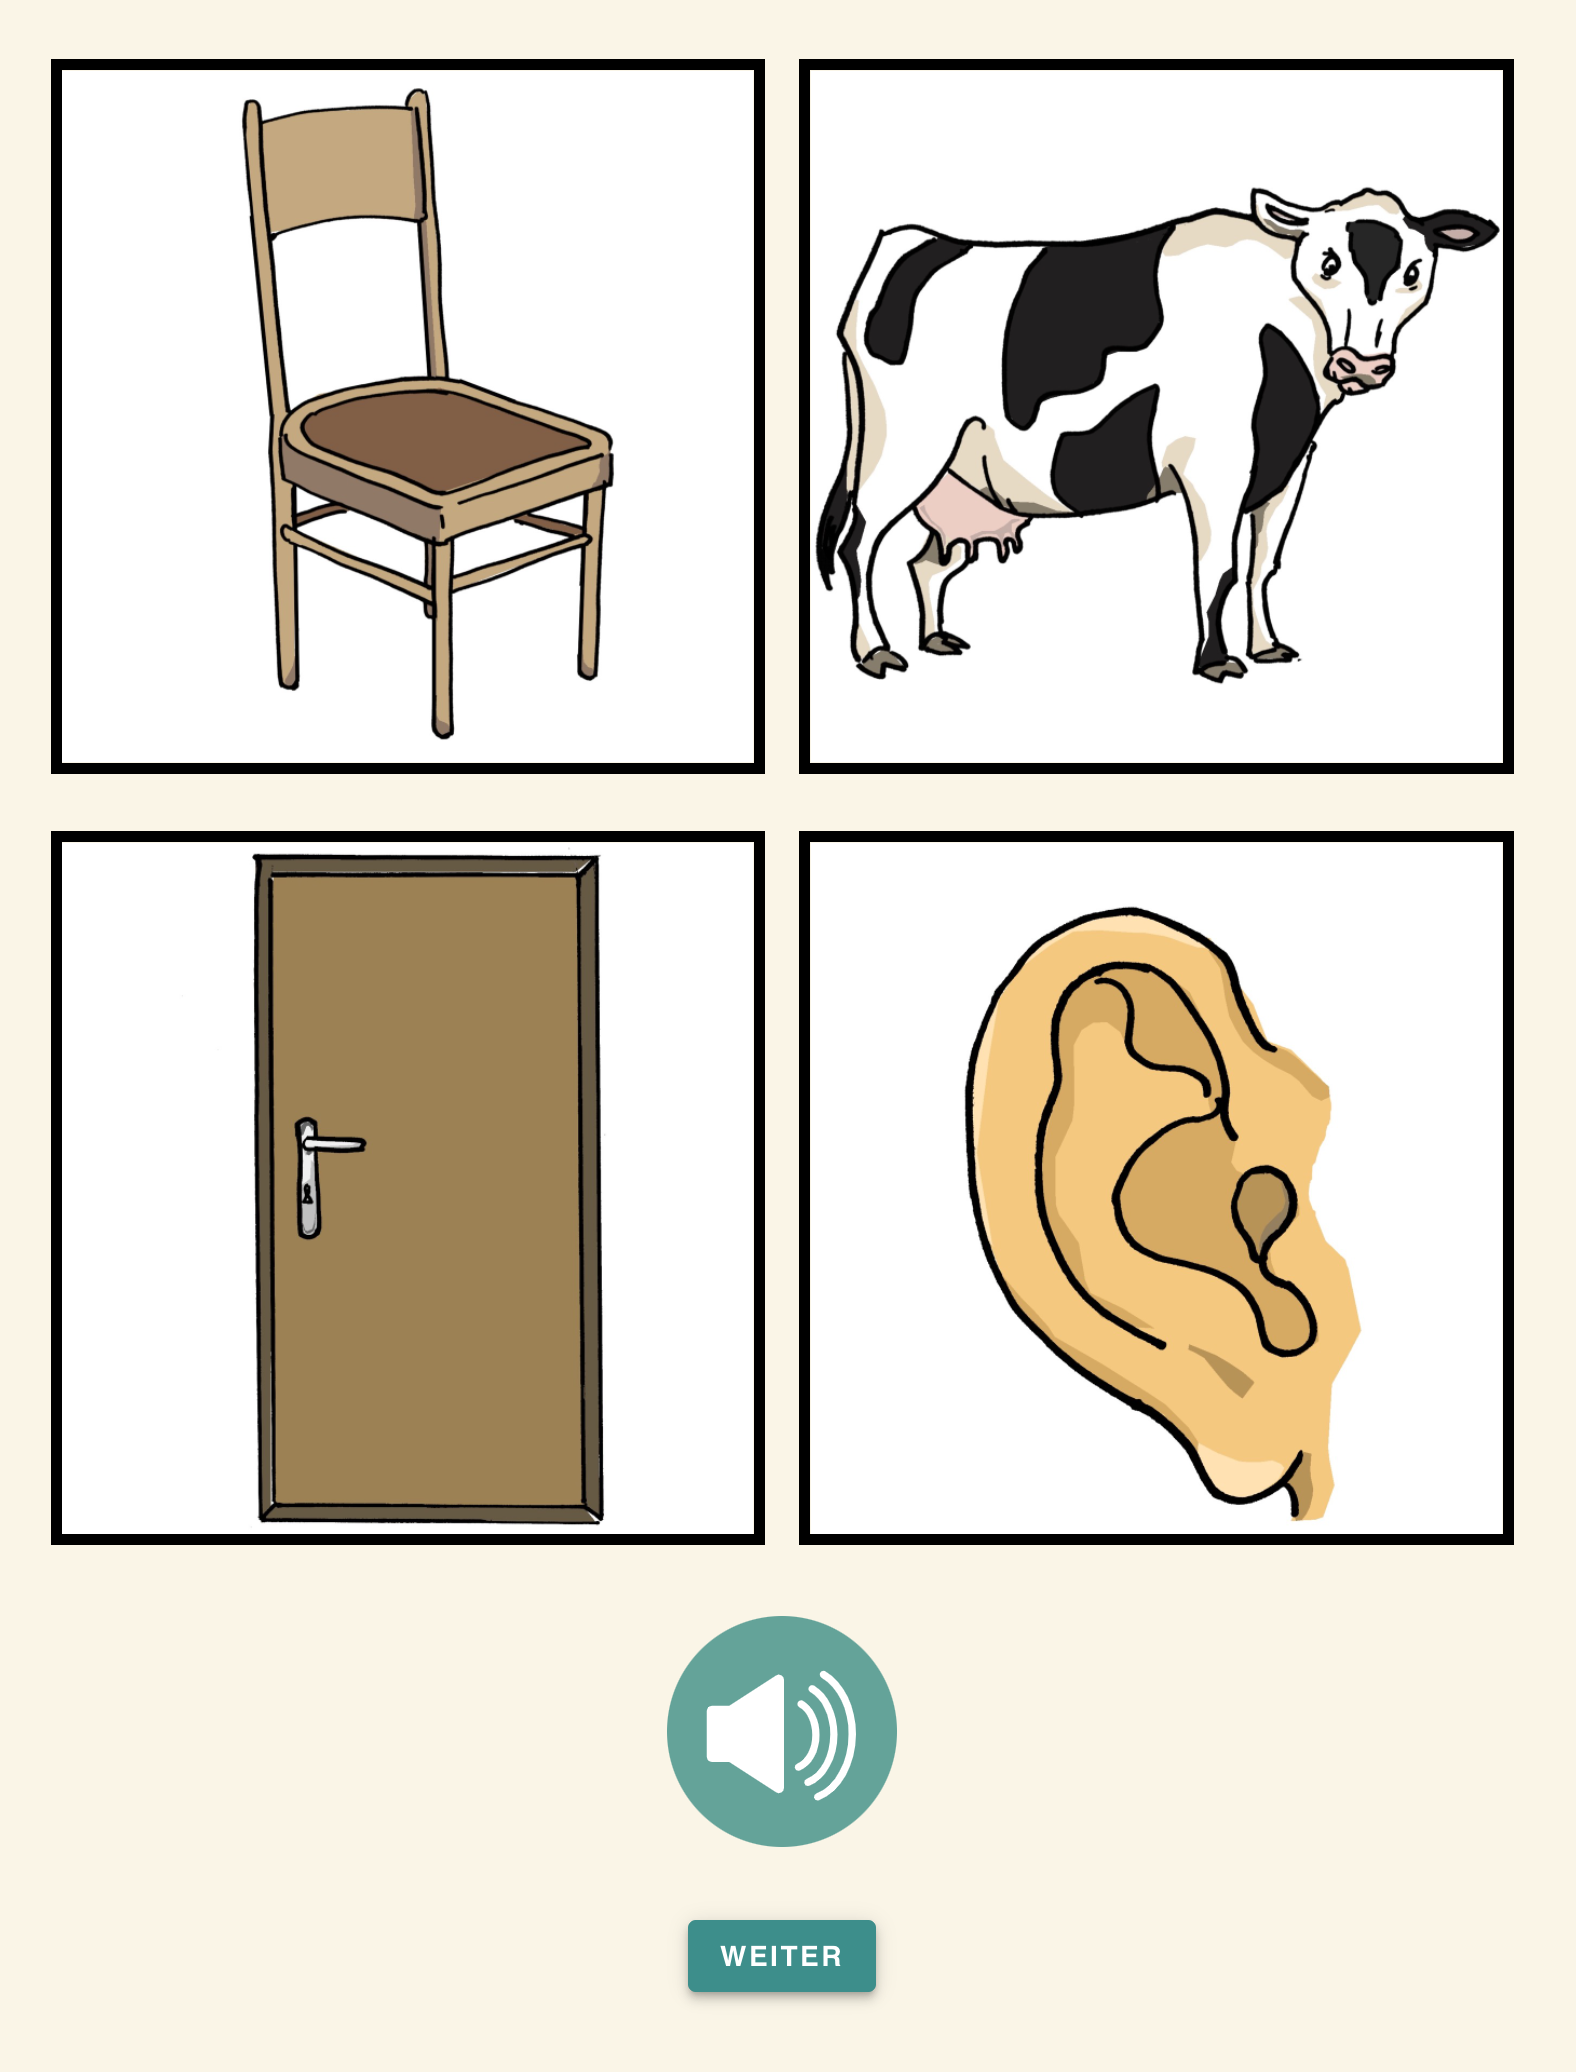
\includegraphics[width=0.5\linewidth]{../graphs/task_fig} 

}

\caption{Screenshot from the task. On each trial, participants heard a word and were asked to pick out the corresponding picture. Verbal prompts could be replayed by pressing the loudspeaker button.}\label{fig:fig1}
\end{figure}

\hypertarget{item-selection}{%
\section{Item selection}\label{item-selection}}

The goal of the item selection process was to find the minimal subset of items necessary to measure vocabulary skills on an individual level. As a first step, we collected data for the full 52-item task from a large sample of children in the target age range. Next, we determined which IRT model best fit the data and used this model to estimate the item parameters (difficulty and discrimination). We removed items that showed differential item functioning (DIF) when the data was split either by sex or by trial order. Finally, we used a simulated annealing process (Kirkpatrick, Gelatt Jr, \& Vecchi, 1983) to determine the size of the reduced tasl and to select the items. Data collection was pre-registered at: \url{https://osf.io/qzstk}. The pre-registered sample size was based on recommendations found in the literature (Morizot, Ainsworth, \& Reise, 2007). The datasets generated during the current study as well as the analysis code are available in the following repository: \url{https://github.com/ccp-eva/vocab}.

\hypertarget{participants}{%
\subsection{Participants}\label{participants}}

Participants were recruited via database of children whose parents volunteered to participate online studies on child development. Parents received and email with a short study description and a personalized link. After one week, parents received a reminder if they had not already taken part in the study. Response rate to invitations was \textasciitilde50\%. The final sample included a total of 581 children (n = 307 girls) with a mean age of 5.63 (range: 3.01 -- 7.99). Participants were randomly assigned to one of the two task versions. Data was collected between February and May 2022.

\hypertarget{descriptive-results}{%
\subsection{Descriptive results}\label{descriptive-results}}



\begin{figure}

{\centering 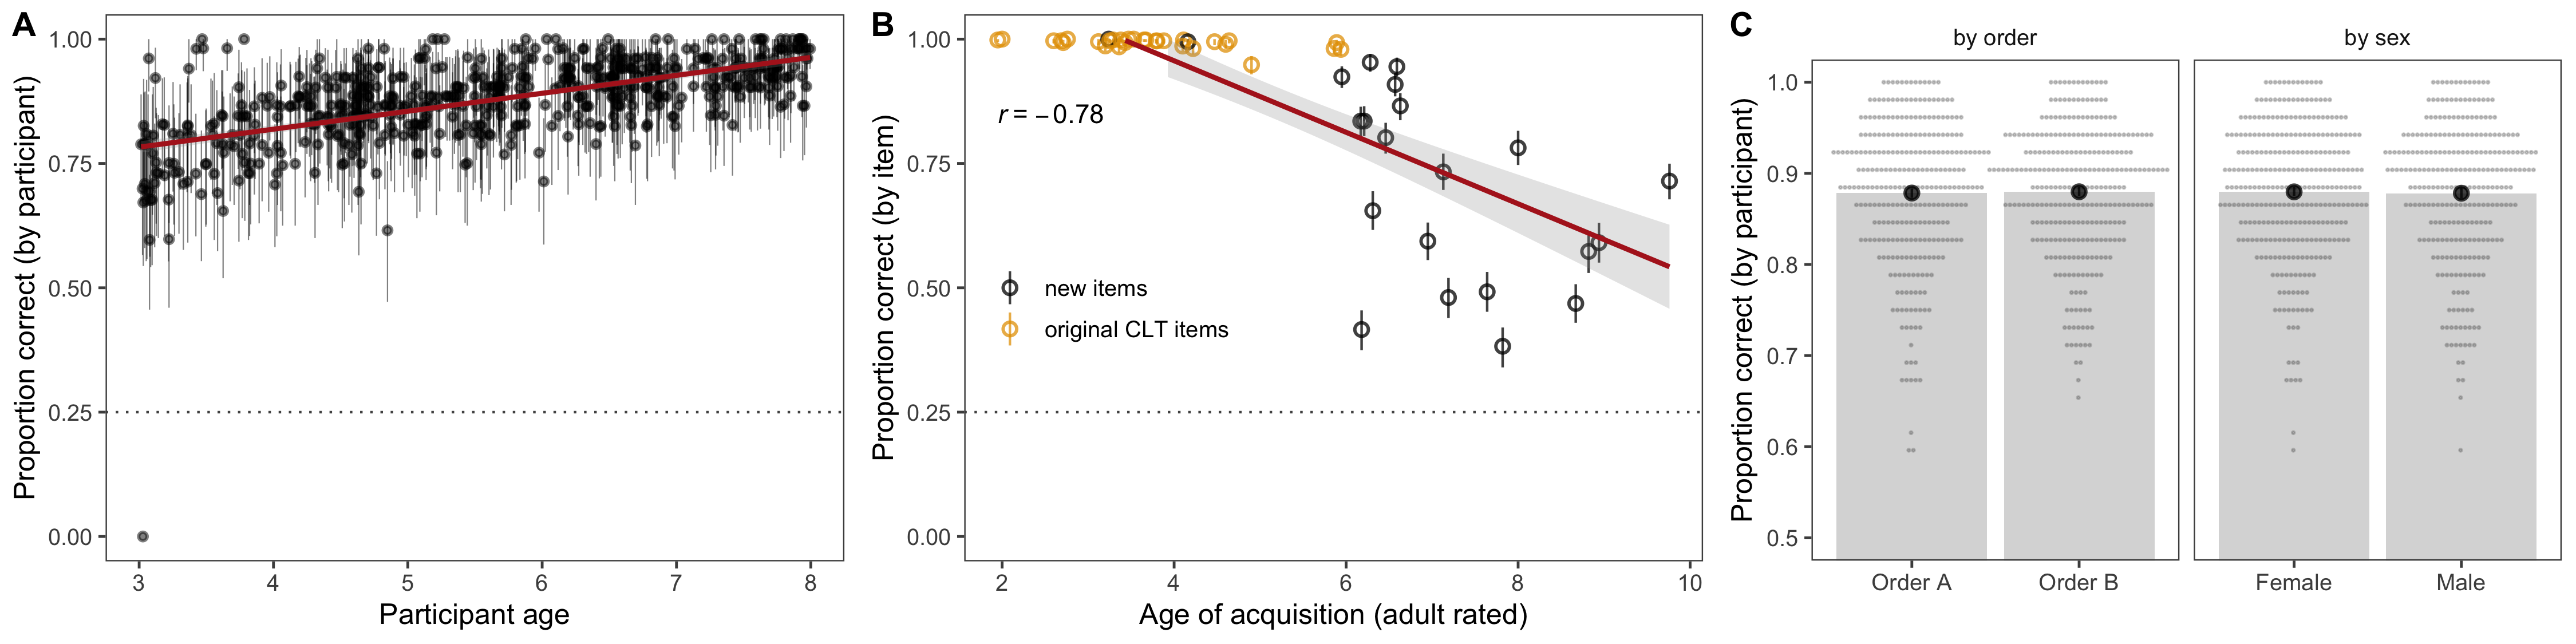
\includegraphics[width=1\linewidth]{../graphs/data_fig} 

}

\caption{Descriptive results of the task. A: Proportion of correct responses (with 95\% CI) for each participant by age. B: Proportion of correct responses (with 95\% CI) for each item by rated age-of-acquisition of the target word. C: Proportion of correct responses (with 95\% CI) by trial order (left) and sex (right).}\label{fig:fig2}
\end{figure}

On a participant level, performance in the full task (52 items) steadily increased with age (Figure \ref{fig:fig2}A). On an item level, performance was above chance (25\%) for all items. Furthermore, the average proportion of correct responses was negatively correlated with age-of-acquisition ratings (Figure \ref{fig:fig2}B). These descriptive results replicate well-known results in the literature and thereby validate the overall approach. Figure \ref{fig:fig2}C shows that there were -- on average -- no differences between participants who received order A and order B as well as between female and male participants. This result suggests that these grouping variables are suitable to investigate differential item functioning (see below).

\hypertarget{item-response-modelling}{%
\subsection{Item response modelling}\label{item-response-modelling}}

IRT models were implemented in a Bayesian framework in \texttt{R} using the \texttt{brms} package (Bürkner, 2017, 2019). Given the binary outcome of the data, we used logistic models to predict the probability of a correct answer based on participant's latent ability and item characteristics (difficulty and discrimination). All models had converging chains and provided a good fit to the data. For details about prior and MCMC settings, please see the analysis script in the associated online repository. We compared models using Bayesian approximate leave-one-out cross-validation (Vehtari, Gelman, \& Gabry, 2017) based on differences in expected log posterior density (ELPD) and the associated standard error (SE).

\begin{table}[tbp]

\begin{center}
\begin{threeparttable}

\caption{\label{tab:tab1}Model comparison}

\begin{tabular}{lllll}
\toprule
Model & ELPD & SE(ELPD) & $\Delta$ELPD & SE($\Delta$ELPD)\\
\midrule
3PL & -6,089.51 & 80.89 & 0.00 & 0.00\\
2PL & -6,124.12 & 81.01 & -34.61 & 8.60\\
1PL (Rasch) & -6,233.70 & 82.13 & -144.19 & 18.20\\
\bottomrule
\addlinespace
\end{tabular}

\begin{tablenotes}[para]
\normalsize{\textit{Note.} ELPD = expected log posterior density, SE = standard error, ELPD differences are in comparison to the 3PL model. Higher ELPD values indicate better model fit.}
\end{tablenotes}

\end{threeparttable}
\end{center}

\end{table}

As a first step, we compared three models with increasing complexity: a 1PL (Rasch) model which assumed that items differ in difficulty but have the same discrimination parameter (1), a 2PL model which addiotionally allowed items to have different discrimination parameters, and a 3Pl model which further added a guessing parameter of 0.25. Table \ref{tab:tab1} shows that the 3PL model provided -- by far -- the best fit. For the following item selection procedure, we therefore used the item parameters (difficulty and discrimination) estimated in the 3PL model.

\hypertarget{differential-item-functioning}{%
\subsection{Differential item functioning}\label{differential-item-functioning}}

\begin{table}[tbp]

\begin{center}
\begin{threeparttable}

\caption{\label{tab:tab2}Model comparison to assess DIF}

\begin{tabular}{lllll}
\toprule
Model & ELPD & SE(ELPD) & $\Delta$ELPD & SE($\Delta$ELPD)\\
\midrule
3PL split by sex & -6,065.58 & 80.94 & 0.00 & 0.00\\
3PL & -6,089.51 & 80.89 & -23.93 & 8.38\\
3PL split by order & -6,090.34 & 80.75 & -24.75 & 9.27\\
\bottomrule
\addlinespace
\end{tabular}

\begin{tablenotes}[para]
\normalsize{\textit{Note.} ELPD = expected log posterior density, SE = standard error, ELPD differences are in comparison to the 3PL model. Higher ELPD values indicate better model fit.}
\end{tablenotes}

\end{threeparttable}
\end{center}

\end{table}

As a first step in the item selection process, we removed items that showed differential item functioning (DIF). DIF refers to situations in which items show differential characteristics for subgroups that have otherwise the same overall score (Holland \& Wainer, 2012). To assess DIF for the present task, we followed the procedure suggested by Bürkner (2019) and fit two extended 3PL models (one for trial order and one for sex) which estimated separate item characteristics for each subgroup. As an overall assessment of DIF we compared these extended models to the basic 3PL. We found no indication for DIF based on trial order but did so for sex (see Table \ref{tab:tab2}). To decide which items to remove, we computed the difference between mean estimates for male and female participants for each item and excluded those items for which the absolute difference was larger than two standard deviations of all differences. Four items had to be excluded based on this procedure (see Figure \ref{fig:fig3}).



\begin{figure}

{\centering 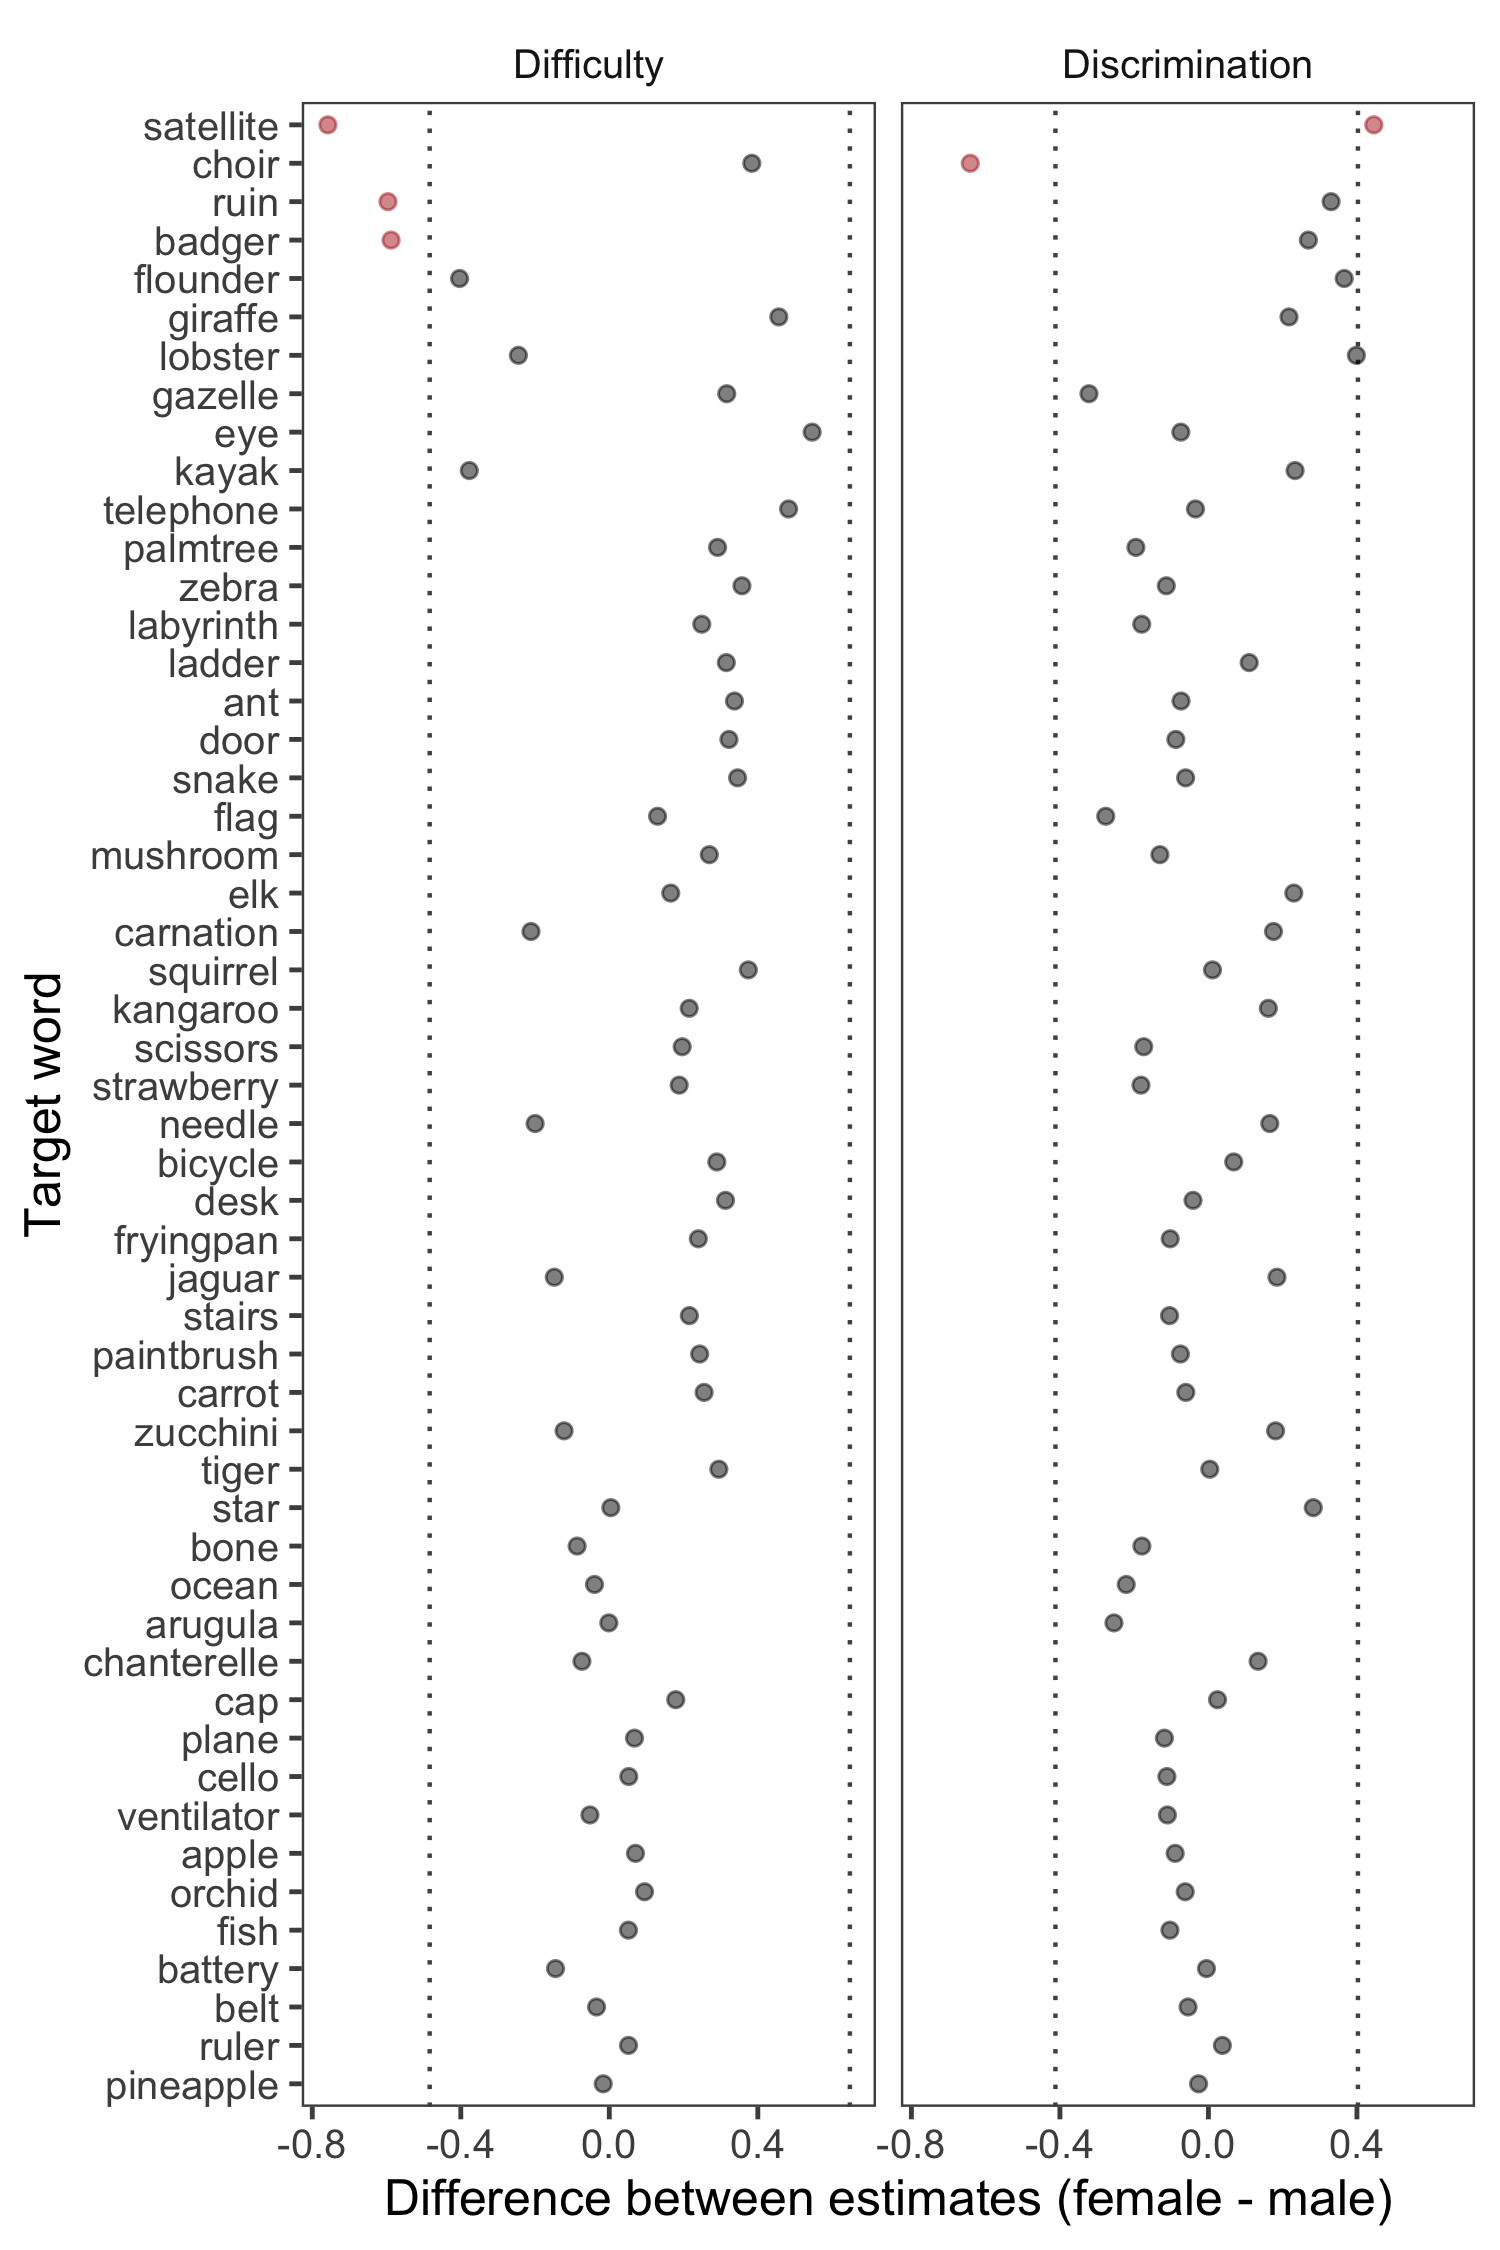
\includegraphics[width=0.5\linewidth]{../graphs/dif_fig} 

}

\caption{Differential item functioning. Difference between estimates for female and male participants for the two item parameters. Dashed lines show cut-off points. Red points indicate items that were excluded.}\label{fig:fig3}
\end{figure}

\hypertarget{simulated-annealing}{%
\subsection{Simulated annealing}\label{simulated-annealing}}

The goal of this last step of the item selection process was to select a smaller subset of items that nevertheless allow for precise measurement. The basis for this selection process was a score which we defined to capture three important characteristics that the items of any subset should have. First, items should be equally spaced across the latent ability space. This characteristic ensures that the task is suited for different ability levels and thus for a broader range of ages. We quantified the spread of any given subset as the standard deviation of the distance (in difficulty estimates) between adjacent items. Lower values indicate smaller distances and thus an overall more equal spacing. Second, items should have maximum discrimination. That is, we preferred items that distinguished well between narrowly defined regions of the latent ability. Discrimination parameters were divided by 2 to put them on a scale comparable to the standard deviations of the distances. Third, difficulty estimates should have narrow credible intervals. The idea behind this characteristic was that many of the easier items had very wide credible intervals because most of the participants answered correctly. Of those items we sought to select the ones with more precise difficulty estimates. For scaling purposes, difficulty estimates were divided by 6.

We used simulated annealing (Kirkpatrick et al., 1983) to find the optimal items for any given size of the subset. This process \ldots{}

We applied simulated annealing to subsets ranging from 5 to 40 items. For each (optimal) subset we then computed the correlation between performance based on the subset and based on the full task This allowed us to assess how well the subset was able to capture variation between individuals in comparison to the full task. Figure \ref{fig:fig4}A shows how the correlation between subset and full task increase with an increasing number of items in the subset. The resulting curve leveled-off at around 20 items in that adding additional items to the subset did not incerease the correlation any further. We therefore concluded that 20 items would be the ideal size of the subset.

When running the simulated annealing procedure for 20 items 100 times, it always returned the same item selection. We therefore chose this subset of items for the reduced task. Figure \ref{fig:fig4}B shows the item parameters for the selected items and Figure \ref{fig:fig4}C shows their item characteristic curves.



\begin{figure}

{\centering 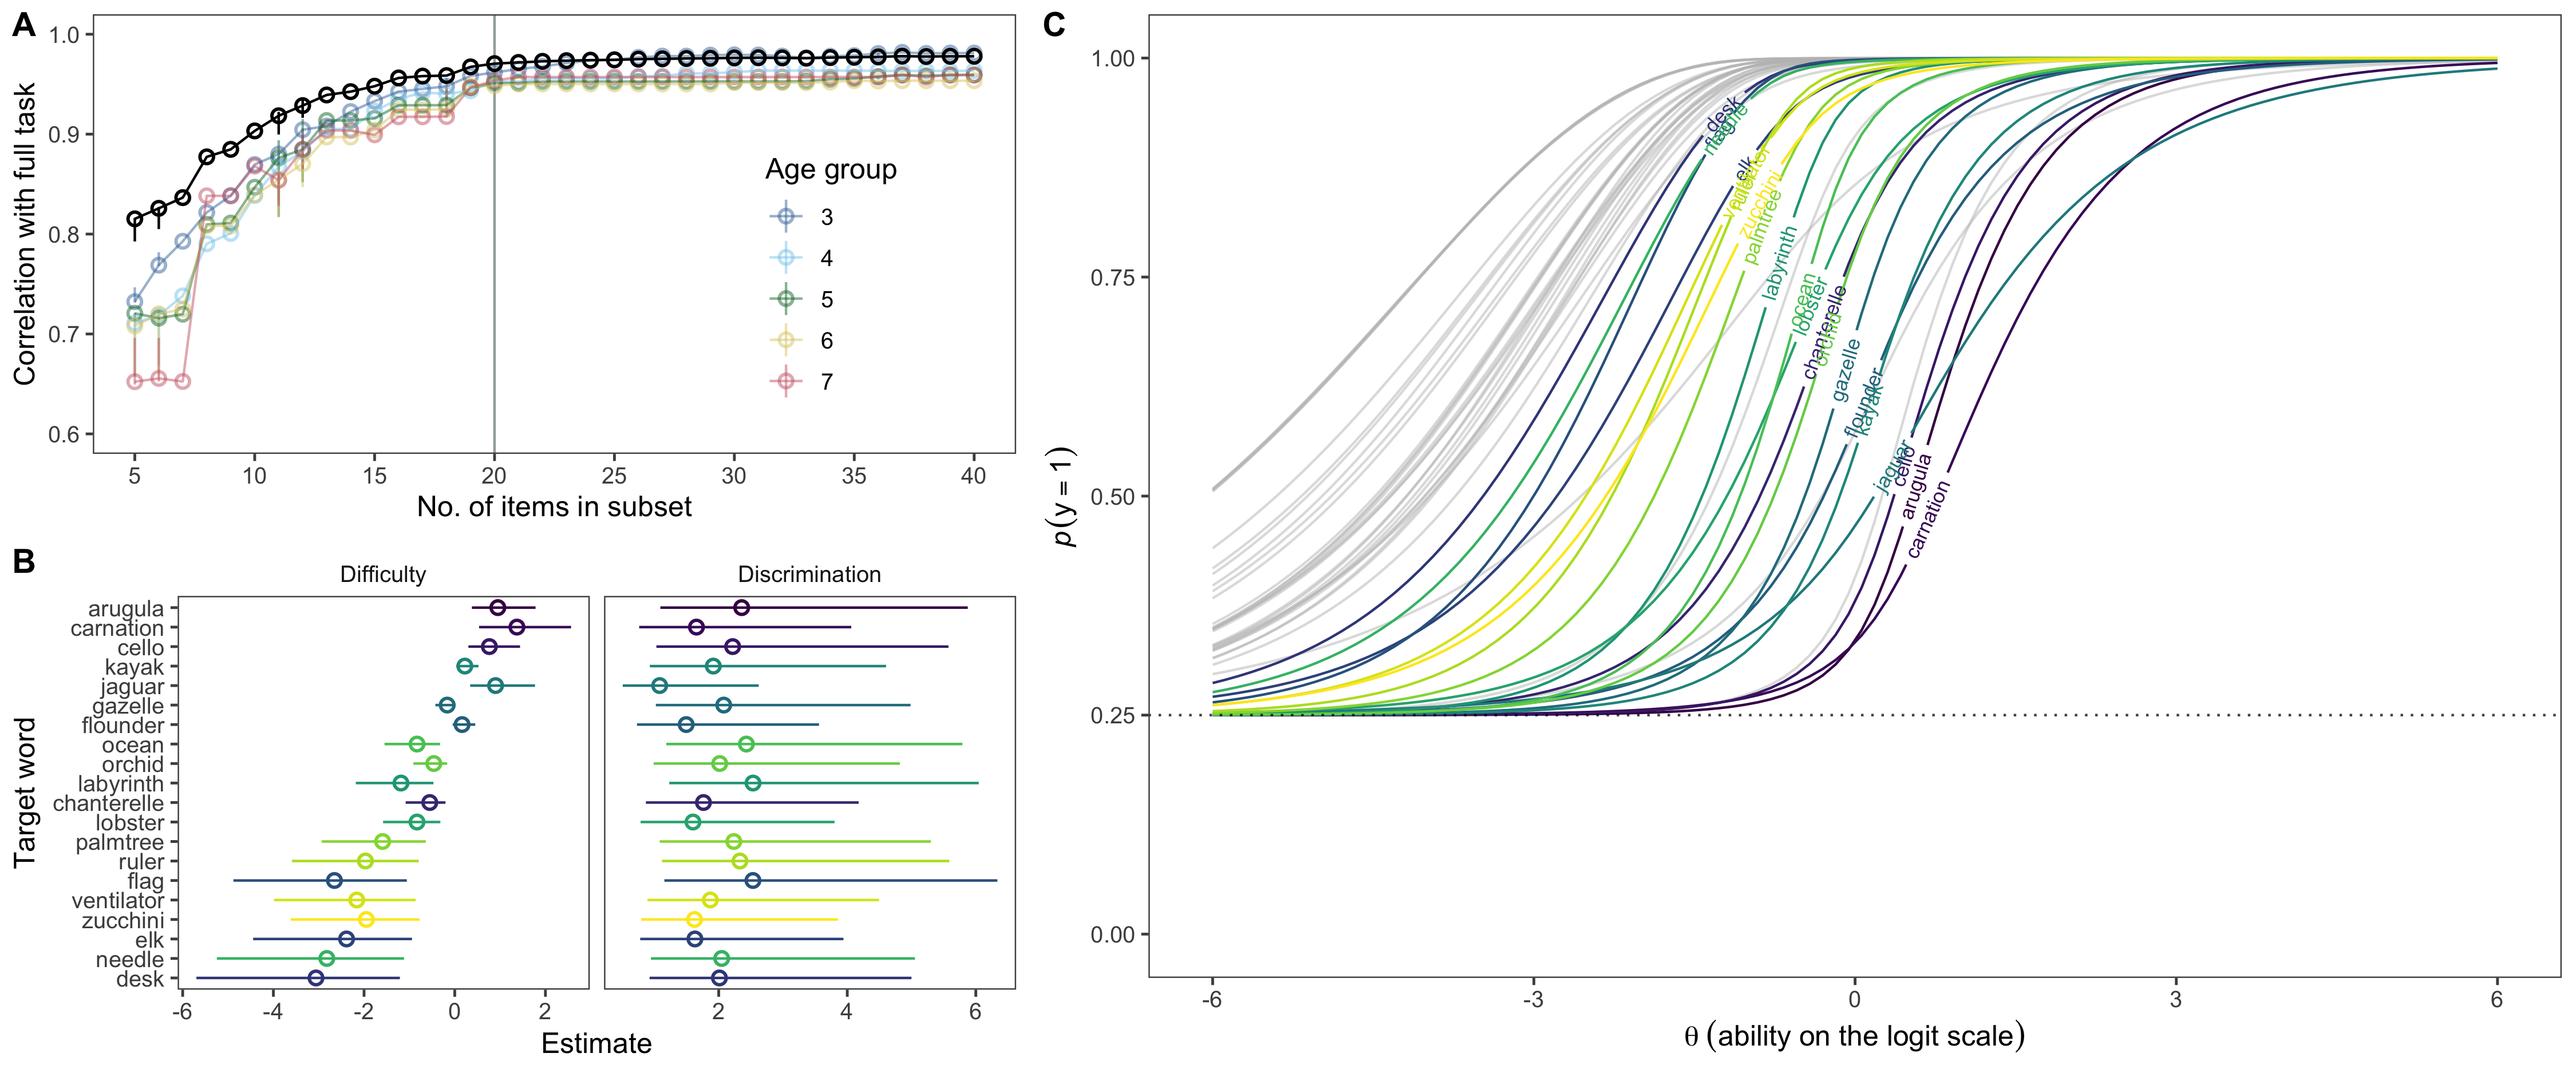
\includegraphics[width=1\linewidth]{../graphs/item_fig2} 

}

\caption{Item selection process. A) Correlation between reduced and full task (52 items). Points show mean correlation based on 100 iterations. Vertical lines show the range of correlations in cases when they differed between iterations. Black lines and points show correlations for the full sample and colored points and lines show correlations by age group. B) Item parameters for the selected 20 items estimated based on the 3PL model. C) Item characteristic curves for all 52 items, with excluded items in grey and selected items in color.}\label{fig:fig4}
\end{figure}

\hypertarget{discussion}{%
\section{Discussion}\label{discussion}}

\newpage

\hypertarget{references}{%
\section{References}\label{references}}

\hypertarget{refs}{}
\begin{CSLReferences}{1}{0}
\leavevmode\vadjust pre{\hypertarget{ref-birchenough2017rated}{}}%
Birchenough, J. M., Davies, R., \& Connelly, V. (2017). Rated age-of-acquisition norms for over 3,200 german words. \emph{Behavior Research Methods}, \emph{49}(2), 484--501.

\leavevmode\vadjust pre{\hypertarget{ref-burkner2017brms}{}}%
Bürkner, P.-C. (2017). Brms: An r package for bayesian multilevel models using stan. \emph{Journal of Statistical Software}, \emph{80}(1), 1--28.

\leavevmode\vadjust pre{\hypertarget{ref-burkner2019bayesian}{}}%
Bürkner, P.-C. (2019). Bayesian item response modeling in r with brms and stan. \emph{arXiv Preprint arXiv:1905.09501}.

\leavevmode\vadjust pre{\hypertarget{ref-dunn1965peabody}{}}%
Dunn, L. M., \& Dunn, L. M. (1965). \emph{Peabody picture vocabulary test}.

\leavevmode\vadjust pre{\hypertarget{ref-haman2017noun}{}}%
Haman, E., Łuniewska, M., Hansen, P., Simonsen, H. G., Chiat, S., Bjekić, J., \ldots{} others. (2017). Noun and verb knowledge in monolingual preschool children across 17 languages: Data from cross-linguistic lexical tasks (LITMUS-CLT). \emph{Clinical Linguistics \& Phonetics}, \emph{31}(11-12), 818--843.

\leavevmode\vadjust pre{\hypertarget{ref-haman2015designing}{}}%
Haman, E., Łuniewska, M., \& Pomiechowska, B. (2015). Designing cross-linguistic lexical tasks (CLTs) for bilingual preschool children. \emph{Assessing Multilingual Children: Disentangling Bilingualism from Language Impairment}, 196--240.

\leavevmode\vadjust pre{\hypertarget{ref-holland2012differential}{}}%
Holland, P. W., \& Wainer, H. (2012). \emph{Differential item functioning}. Routledge.

\leavevmode\vadjust pre{\hypertarget{ref-kirkpatrick1983optimization}{}}%
Kirkpatrick, S., Gelatt Jr, C. D., \& Vecchi, M. P. (1983). Optimization by simulated annealing. \emph{Science}, \emph{220}(4598), 671--680.

\leavevmode\vadjust pre{\hypertarget{ref-luniewska2019age}{}}%
Łuniewska, M., Wodniecka, Z., Miller, C. A., Smolik, F., Butcher, M., Chondrogianni, V., \ldots{} others. (2019). Age of acquisition of 299 words in seven languages: American english, czech, gaelic, lebanese arabic, malay, persian and western armenian. \emph{PloS One}, \emph{14}(8), e0220611.

\leavevmode\vadjust pre{\hypertarget{ref-morizot2007toward}{}}%
Morizot, J., Ainsworth, A., \& Reise, S. (2007). \emph{Toward modern psychometrics: Application of item response theory models in personality research in robins RW, fraley RC, \& krueger RF (eds.), Handbook of research methods in personality psychology (pp. 407--421)}. New York, NY: Guildford Press.{[}Google Scholar{]}.

\leavevmode\vadjust pre{\hypertarget{ref-schroder2012german}{}}%
Schröder, A., Gemballa, T., Ruppin, S., \& Wartenburger, I. (2012). German norms for semantic typicality, age of acquisition, and concept familiarity. \emph{Behavior Research Methods}, \emph{44}(2), 380--394.

\leavevmode\vadjust pre{\hypertarget{ref-vehtari2017practical}{}}%
Vehtari, A., Gelman, A., \& Gabry, J. (2017). Practical bayesian model evaluation using leave-one-out cross-validation and WAIC. \emph{Statistics and Computing}, \emph{27}(5), 1413--1432.

\end{CSLReferences}


\end{document}
